\documentclass{article}

% packages
\usepackage{amsmath, amsthm, thmtools, amsfonts, amssymb, luacode, catchfile, tikzducks, hyperref, ifthen}
\ifcsname c@kobocompile\endcsname
	\usepackage[a5paper, total={1072pt, 1448pt}, margin=10pt, includeheadfoot]{geometry} % set page margins
\else
	\usepackage[a4paper, margin=50pt, includeheadfoot]{geometry}
\fi
\usepackage[shortlabels]{enumitem}
\usepackage[skip=3pt, indent=0pt]{parskip}

% language
\usepackage[bidi=basic, layout=tabular, provide=*]{babel}
\ifcsname c@english\endcsname
	\babelprovide[main, import]{english}
\else
	\babelprovide[main, import]{hebrew}
	\babelprovide{rl}
\fi
%\babelfont{rm}{Libertinus Serif}
\babelfont{rm}[Renderer=Harfbuzz]{Libertinus Serif}
\babelfont{sf}{Libertinus Sans}
\babelfont{tt}{Libertinus Mono}

% style
\AddToHook{cmd/section/before}{\clearpage}	% Add line break before section
\linespread{1.3}
\setcounter{secnumdepth}{0}		% Remove default number tags from sections, this won't do well with theorems
\AtBeginDocument{\setlength{\belowdisplayskip}{3pt}}
\AtBeginDocument{\setlength{\abovedisplayskip}{3pt}}
\graphicspath{ {../images/} }

% operators
\DeclareMathOperator\cis{cis}
\DeclareMathOperator\Sp{Sp}
\DeclareMathOperator\tr{tr}
\DeclareMathOperator\im{Im}
\DeclareMathOperator\re{Re}
\DeclareMathOperator\diag{diag}
\DeclareMathOperator*\lowlim{\underline{lim}}
\DeclareMathOperator*\uplim{\overline{lim}}
\DeclareMathOperator\rng{rng}
\DeclareMathOperator\Sym{Sym}
\DeclareMathOperator\Arg{Arg}
\DeclareMathOperator\Log{Log}
\DeclareMathOperator\dom{dom}
\DeclareMathOperator\supp{Supp}
\DeclareMathOperator\var{Var}
\DeclareMathOperator\cov{Cov}

% commands
%\renewcommand\qedsymbol{\textbf{מש''ל}}
%\renewcommand\qedsymbol{\fbox{\emoji{lizard}}}
\newcommand{\Aa}[0]{\mathcal{A}}
\newcommand{\Bb}[0]{\mathcal{B}}
\newcommand{\CC}[0]{\mathbb{C}}
\newcommand{\Cc}[0]{\mathcal{C}}
\newcommand{\EE}[0]{\mathbb{E}}
\newcommand{\FF}[0]{\mathbb{F}}
\newcommand{\Ff}[0]{\mathcal{F}}
\newcommand{\Ii}[0]{\mathcal{I}}
\newcommand{\Gg}[0]{\mathcal{G}}
\newcommand{\Ll}[0]{\mathcal{L}}
\newcommand{\Mm}[0]{\mathcal{M}}
\newcommand{\NN}[0]{\mathbb{N}}
\newcommand{\Nn}[0]{\mathcal{N}}
\newcommand{\PP}[0]{\mathbb{P}}
\newcommand{\Pp}[0]{\mathcal{P}}
\newcommand{\QQ}[0]{\mathbb{Q}}
\newcommand{\RR}[0]{\mathbb{R}}
\newcommand{\Rr}[0]{\mathcal{R}}
\newcommand{\Ss}[0]{\mathcal{S}}
\newcommand{\TT}[0]{\mathbb{T}}
\newcommand{\Uu}[0]{\mathcal{U}}
\newcommand{\Vv}[0]{\mathcal{V}}
\newcommand{\Ww}[0]{\mathcal{W}}
\newcommand{\ZZ}[0]{\mathbb{Z}}
\newcommand{\acts}[0]{\circlearrowright}
\newcommand{\explain}[2] {
	\begin{flalign*}
		 && \text{#2} && \text{#1}
	\end{flalign*}
}
\newcommand{\maketitleprint}[0]{ \begin{center}
	%\begin{tikzpicture}[scale=3]
	%	\duck[graduate=gray!20!black, tassel=red!70!black]
	%\end{tikzpicture}	
	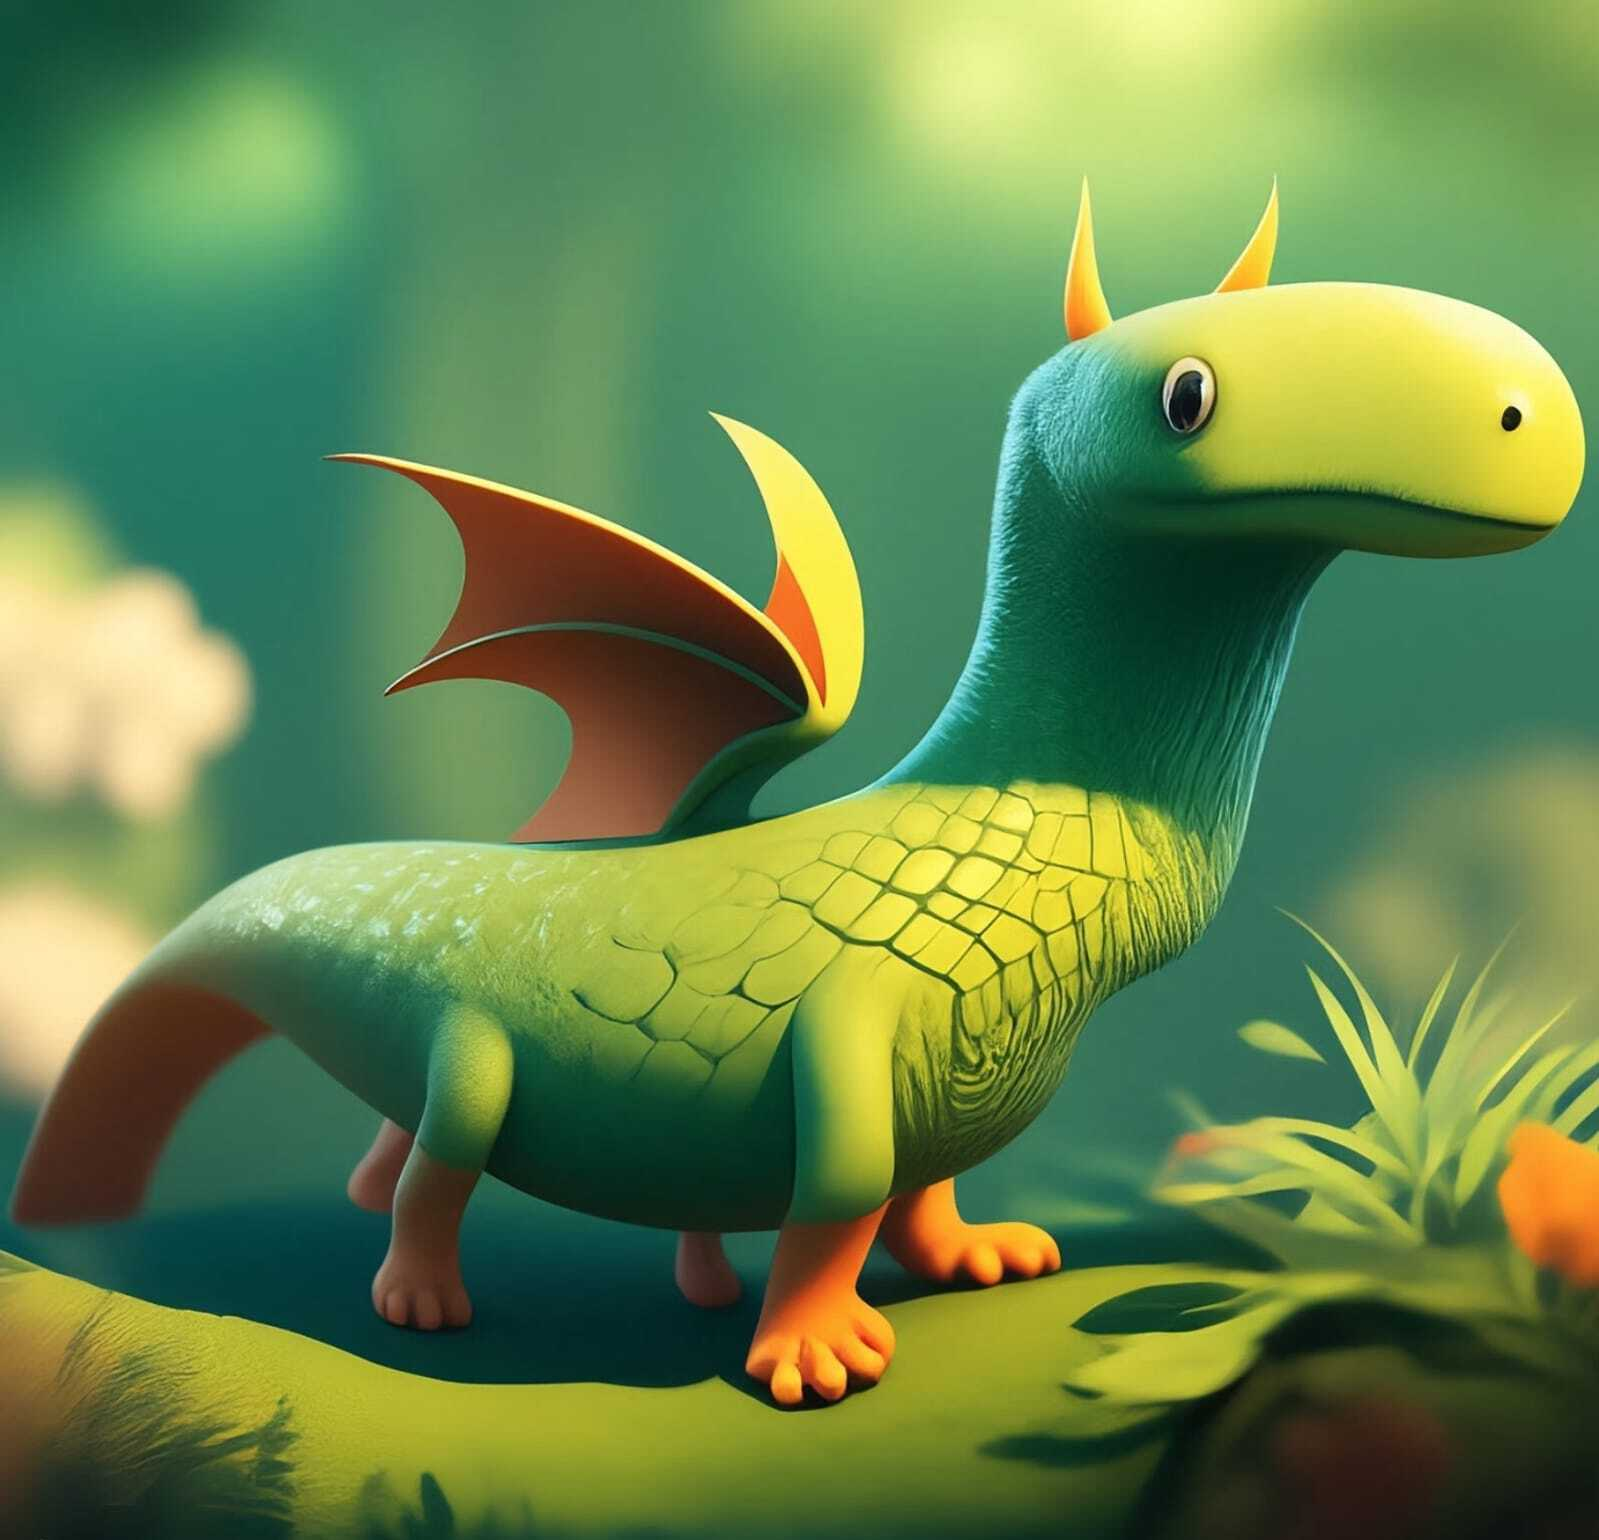
\includegraphics[width=6cm]{cover}
\end{center}
}

% theorem commands
\newtheoremstyle{c_remark}
	{}	% Space above
	{}	% Space below
	{}% Body font
	{}	% Indent amount
	{\bfseries}	% Theorem head font
	{}	% Punctuation after theorem head
	{.5em}	% Space after theorem head
	{\thmname{#1}\thmnumber{ #2}\thmnote{ \normalfont{\text{(#3)}}}}	% head content
\newtheoremstyle{c_definition}
	{3pt}	% Space above
	{3pt}	% Space below
	{}% Body font
	{}	% Indent amount
	{\bfseries}	% Theorem head font
	{}	% Punctuation after theorem head
	{.5em}	% Space after theorem head
	{\thmname{#1}\thmnumber{ #2}\thmnote{ \normalfont{\text{(#3)}}}}	% head content
\newtheoremstyle{c_plain}
	{3pt}	% Space above
	{3pt}	% Space below
	{\itshape}% Body font
	{}	% Indent amount
	{\bfseries}	% Theorem head font
	{}	% Punctuation after theorem head
	{.5em}	% Space after theorem head
	{\thmname{#1}\thmnumber{ #2}\thmnote{ \text{(#3)}}}	% head content

\ifcsname c@english\endcsname
	\theoremstyle{plain}
	\newtheorem{theorem}{Theorem}[section]
	\newtheorem{lemma}[theorem]{Lemma}
	\newtheorem{proposition}[theorem]{Proposition}
	\newtheorem*{proposition*}{Proposition}
	%\newtheorem{corollary}[theorem]{אין חלופה עברית}

	\theoremstyle{definition}
	\newtheorem{definition}[theorem]{Definition}
	\newtheorem*{definition*}{Definition}
	\newtheorem{example}{Example}[section]
	\newtheorem{exercise}{Exercise}[section]

	\theoremstyle{remark}
	\newtheorem*{remark}{Remark}
	\newtheorem*{solution}{Solution}
	\newtheorem{conclusion}[theorem]{Conclusion}
	\newtheorem{notation}[theorem]{Notation}
\else
	\theoremstyle{c_plain}
	\newtheorem{theorem}{משפט}[section]
	\newtheorem{lemma}[theorem]{למה}
	\newtheorem{proposition}[theorem]{טענה}
	\newtheorem*{proposition*}{טענה}
	%\newtheorem{corollary}[theorem]{אין חלופה עברית}

	\theoremstyle{c_definition}
	\newtheorem{definition}[theorem]{הגדרה}
	\newtheorem*{definition*}{הגדרה}
	\newtheorem{example}{דוגמה}[section]
	\newtheorem{exercise}{תרגיל}[section]

	\theoremstyle{c_remark}
	\newtheorem*{remark}{הערה}
	\newtheorem*{solution}{פתרון}
	\newtheorem{conclusion}[theorem]{מסקנה}
	\newtheorem{notation}[theorem]{סימון}
\fi

% Questions related commands
\newcounter{question}
\setcounter{question}{1}
\newcounter{sub_question}
\setcounter{sub_question}{1}

\ifcsname c@english\endcsname
	\newcommand{\question}[1][0]{
		\ifthenelse{#1 = 0}{}{\setcounter{question}{#1}}
		\section{Question \arabic{question}}
		\addtocounter{question}{1}
		\setcounter{sub_question}{1}
	}

	\newcommand{\subquestion}[1][0]{
		\ifthenelse{#1 = 0}{}{\setcounter{sub_question}{#1}}
		\subsection{Part \alph{sub_question}}
		\addtocounter{sub_question}{1}
	}
\else
	\newcommand{\question}[1][0]{
		\ifthenelse{#1 = 0}{}{\setcounter{question}{#1}}
		\section{שאלה \arabic{question}}
		\addtocounter{question}{1}
		\setcounter{sub_question}{1}
	}

	\newcommand{\subquestion}[1][0]{
		\ifthenelse{#1 = 0}{}{\setcounter{sub_question}{#1}}
		\subsection{סעיף \localecounter{letters.gershayim}{sub_question}}
		\addtocounter{sub_question}{1}
	}
\fi

% import lua and start of document
\directlua{common = require ('../common')}

\GetEnv{AUTHOR}

% headers
\author{\AUTHOR}
\date\today

\title{פתרון מטלה 03 --- מבוא לטופולוגיה, 80516}
% chktex-file 9
% chktex-file 17

\begin{document}
\maketitle
\maketitleprint{}

\question[2]
בכל אחד מן הסעיפים הבאים נגדיר מרחב טופולוגי $(X, \tau)$ ותת־קבוצה $A \subseteq X$ ונמצא את $A^\circ, \partial A$.

\subquestion{}
נגדיר $X = \RR, \Bb_{\tau} = \{ [a, b) \mid a, b \in \RR \}$, כלומר הישר של זורגנפריי,  יחד עם $A = (0, 1]$.
\begin{solution}
	נבחין כי $\{ [a, b) \mid 0 < a < b < 1 \} \subseteq \Bb_{\tau}$ היא קבוצת איברי הבסיס החלקיים ל־$A$, ולכן גם כל קבוצה $U \subseteq A$ פתוחה היא איחוד מהקבוצה שהצגנו,
	נובע אם כך מהגדרה שמתקיים,
	\[
		A^\circ
		= \bigcup \{ [a, b) \mid 0 < a < b \le 1 \}
		= (0, 1)
	\]
	נבחן עתה את ${(A^C)}^\circ$.
	אנו יודעים ש־$A^C = (-\infty, 0] \cup (1, \infty)$, ונוכל מהליך זהה לזה שעשינו עבור הקבוצה המקורית לקבוע כי ${(A^C)}^\circ = (-\infty, 0) \cup (1, \infty)$, ולכן $\overline{A} = [0, 1]$.
	נסיק ש־$\partial A = \{0, 1\}$.
\end{solution}

\subquestion{}
נגדיר $X = \RR$ עם הטופולוגיה הקו־סופית, והקבוצה $A = [0, 1)$.
\begin{solution}
	נתחיל ונבחין ש־$|A| = |\RR|$, לכן $A \in \tau$, כלומר $A = A^\circ$.
	בטופולוגיה הקו־סופית כל קבוצה סגורה היא מגודל סופי או $X$, לכן לא קיימת קבוצה סגורה מלבד $X$ כך שהיא מכילה את $A$, נסיק אם כן ש־$\overline{A} = \RR$.
	לבסוף נובע ש־$\partial A = A^C$.
\end{solution}

\subquestion{}
נגדיר $X = C[0, 1]$ יחד עם מטריקת סופרימום, ונגדיר את $\tau$ להיות הטופולוגיה המושרית ממטריקה זו. \\
נגדיר גם $A = \{ f \in C[0, 1] \mid \exists x \in [0, 1], f(x) \in [0, 1] \}$.
\begin{solution}
	תהי $f \in A$, נרצה להבין אם $f \in A^\circ$.
	אנו רוצים לבחון אם קיים $\epsilon > 0$ כך ש־$B(f, \rho) \subseteq A$.
	אם $g \in B(f, \epsilon)$ אז לכל $x \in [0, 1]$ מתקיים $|f(x) - g(x)| < \epsilon$, ולכן אם $f(x) \in (0, 1)$ עבור איזשהו $x$, אז בהכרח קיים $\epsilon$ כזה.
	אילו $f(x) \in \{0, 1\}$ עבור איזשהו $x$ בלבד ו־$f(x) \notin (0, 1)$, אז תמיד נוכל לבחור $g(x) = f(x) + \epsilon$ ונקבל ש־$g \notin A$.
	נסיק שמתקיים,
	\[
		A^\circ
		= \{ f \in C[0, 1] \mid \exists x \in [0, 1], f(x) \in (0, 1) \}
	\]
	נטען גם ש־$A$ קבוצה סגורה, זאת שכן $A^C = \{ f \in C[0, 1] \mid \forall x, f(x) \notin [0, 1] \}$, ומשיקולים דומים קיים כדור מוכל סביב כל פונקציה בקבוצה זו.
	לכן נסיק,
	\[
		\partial A
		= \{ f \in X \mid \exists x \in [0, 1], f(x) \in \{0, 1\}, \forall y, f(y) \notin (0, 1) \}
	\]
\end{solution}

\question{}
יהיו $(X, \tau), (Y, \sigma)$ מרחבים טופולוגיים ותהי $f : X \to Y$ העתקת מנה.
נניח ש־$\sim_f$ יחס השקילות על $X$ המוגדר על־ידי $x \sim_f Y \iff f(x) = f(y)$.
נסמן ב־$p$ את ההטלה של $X$ ל־$X / \sim_f$.
נוכיח כי קיים ויחיד הומיאומורפיזם $i : (Y, \sigma) \to (X / \sim_f, p_* \tau)$ כך ש־$i \circ f = p$.
\begin{proof}
	נגדיר $i$ כזה.
	לכל $y \in Y$ יהי $x \in X$ כך ש־$f(x) = y$, ידוע כי $f$ על ולכן יש כזה.
	נגדיר אם כך $i(y) = {[x]}_{\sim_f}$.
	נבחין כי הגדרה זו לא תלויה בבחירת $x$, שכן אם $f(x') = y$ גם כן, אז $[x] = [x']$.
	זוהי אם כן גם העתקה חד־חד ערכית, אחרת נקבל ש־$f$ לא מקיימת את תנאי הפונקציה, וכן $i$ על ישירות מהגדרת יחס השקילות $\sim_f$.
	לבסוף ישירות מהגדרת העתקת מנה נסיק ש־$i$ היא העתקה פתוחה ורציפה, ולכן גם הומיאומורפיזם.

	עתה נרצה להוכיח ש־$i$ מקיימת את הטענה האמורה, וכי אם $j$ הומיאומורפיזם המקיים את הדרישה אף הוא, אז $i = j$.
	יהי $x \in X$, אז $i(f(x)) = {[x]}_{\sim_f} = p(x)$ ישירות מהגדרה.
	לכל $y \in Y$ קיים $x \in X$ כך ש־$i(y) = [x]$, לכן גם $j(f(x)) = j(y) = [x]$, וקיבלנו $i(x) = j(x)$, ונסיק $i = j$.
	לכן $i$ הומיאומורפיזם יחיד.
\end{proof}

\question{}
בשאלה זו נעסוק ב־$\RR P^n$.

\subquestion{}
נוכיח כי $\RR P^1$ הומיאומורפי ל־$S^1$.
\begin{proof}
	מטעמי נוחות נבחן את שני המרחבים מעל המרוכבים, נניח ש־$z \in \CC \setminus \{0\}$, אז $[z] = \{ t z \mid t \in \RR \setminus \{0\}\}$.
	נגדיר $f([z]) = z^2$ עבור הנציג המקיים $|z| = 1$. נבחין כי זוהי הגדרה עקבית, זאת שכן אם $z \sim w$ אבל $z \ne w$, אז $|z| = |w| = 1$ וכן $-z = w$, אז $z^2 = w^2$.
	העתקה זו כמובן גם חד־חד ערכית כפולינום מרוכב ועל מאותה הסיבה.
	זוהי גם העתקה רציפה ל־$\CC$ ולכן גם לצמצום של המרחב.

	נרצה אם כך להראות שהיא פתוחה.
	נניח ש־$U^* \subseteq \RR P^1$ קבוצה פתוחה, אז נבחר את $U \subseteq \CC$ קבוצת הנציגים של $U^*$ כך ש־$\forall x \in U, |x| = 1$.
	נגדיר גם ש־$x, -x \in U$, ונקבל קבוצה פתוחה ב־$\CC$, ולכן תמונתה פתוחה אף היא ב־$\CC$ וכן צמצומה פתוח.
	נסיק ש־$f$ היא הומיאומורפיזם.
\end{proof}

\subquestion{}
יהי $n \in \NN$, נראה ש־$\RR P^n$ הוא מנה של $S^n$.
\begin{proof}
	נגדיר את ההעתקה $f : S^n \to \RR P^n$ על־ידי $f([x]) = \{ t x \mid t \in \RR \setminus \{0\}\}$.
	זוהי העתקה מוגדרת היטב מטעמי כיסוי כל הנציגים בישר, והיא על ישירות מבחירת נציג בטווח.

	אנו רוצים להראות כי $U \subseteq \RR P^n$ היא פתוחה אם ורק אם $f^{-1}(U)$ פתוחה.
	הטופולוגיות על שני המרחבים בנויים על מנה של $\RR^{n + 1}$, ולכן אם $U$ קבוצה פתוחה אז בהכרח $\bigcup [U]$ פתוחה ב־$\RR^{n + 1}$, אבל במקרה זה נובע ישירות ש־$\bigcup [U] / \sim$ עבור היחס המשרה את $S^n$ פתוחה אף היא.
	נסיק כי אכן מתקיימת הדרישה, ולכן $\RR P^n$ הוא מנה של $S^n$.
\end{proof}

\end{document}
